% !TEX root = main.tex
\chapter{Simulações e Resultados}
\label{cha:results}

A fim de melhorar as condições de reprodutibilidade das simulações realizadas neste trabalho, é importante observar a Tabela \ref{tab:results_pc_specs}, que traz as configurações do ambiente em que todas as simulações foram realizadas.

\begin{table}[H]
    \centering
    \caption{Ambiente de simulação.}
    \begin{tabular}{ll}
        \toprule
        \textbf{Componente} &   \textbf{Descrição}\\
        \midrule
        Processador         &   Intel Core i5-8600K 3.6 GHz (4.3 GHz Turbo) 6-Core 9 MB Cache\\
        Cooler              &   Corsair H80i v2 Water Cooler\\
        Placa Mãe           &   Gigabyte Z370XP SLI\\
        Memória RAM         &   Corsair Vengeance DDR4 3000 MHz 16 GB (2 x 8 GB) C15\\
        SSD                 &   Kingston UV400 240 GB SATA III\\
        SSHD                &   Seagate Híbrido Firecuda 2 TB 64 MB Cache SATA III\\
        Placa de Vídeo      &   EVGA GTX 1080 Ti SC2 11 GB\\
        Fonte               &   Corsair CS750M\\
        Sistema Operacional &   Ubuntu Desktop 18.04 LTS 64-bit\\
        CUDA                &   v10.0\\
        CUDNN               &   v7.5\\
        PyTorch             &   v1.0.1\\
        \bottomrule
    \end{tabular}
    \label{tab:results_pc_specs}
\end{table}






\begin{figure}[H]
    \centering
    \subfigure[Época 0]
    {
        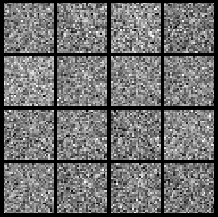
\includegraphics[width=0.30\textwidth]{figs/MNIST/new_tests/_epoch_0_batch_0.png}
        \label{fig:results_mnist_epoch-0}
    }
    \hspace{0.5cm}
    \subfigure[Época 3]
    {
        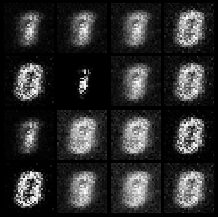
\includegraphics[width=0.30\textwidth]{figs/MNIST/new_tests/_epoch_3_batch_500.png}
        \label{fig:results_mnist_epoch-3}
    }
    \\
    \vspace{0.5cm}
    \subfigure[Época 32]
    {
        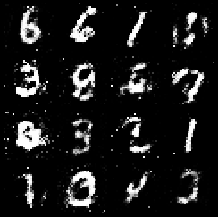
\includegraphics[width=0.30\textwidth]{figs/MNIST/new_tests/_epoch_32_batch_400.png}
        \label{fig:results_mnist_epoch-32}
    }
    \hspace{0.5cm}
    \subfigure[Época 299]
    {
        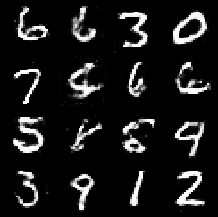
\includegraphics[width=0.30\textwidth]{figs/MNIST/new_tests/_epoch_299_batch_500.png}
        \label{fig:results_mnist_epoch-299}
    }
    \caption{Gerações da GAN \textit{Vanilla} para o \textit{dataset} MNIST em diferentes épocas.}
    \label{fig:results_mnist}
\end{figure}



\pagebreak
\newpage



\begin{figure}[H]
    \centering
    \subfigure[Erros]
    {
        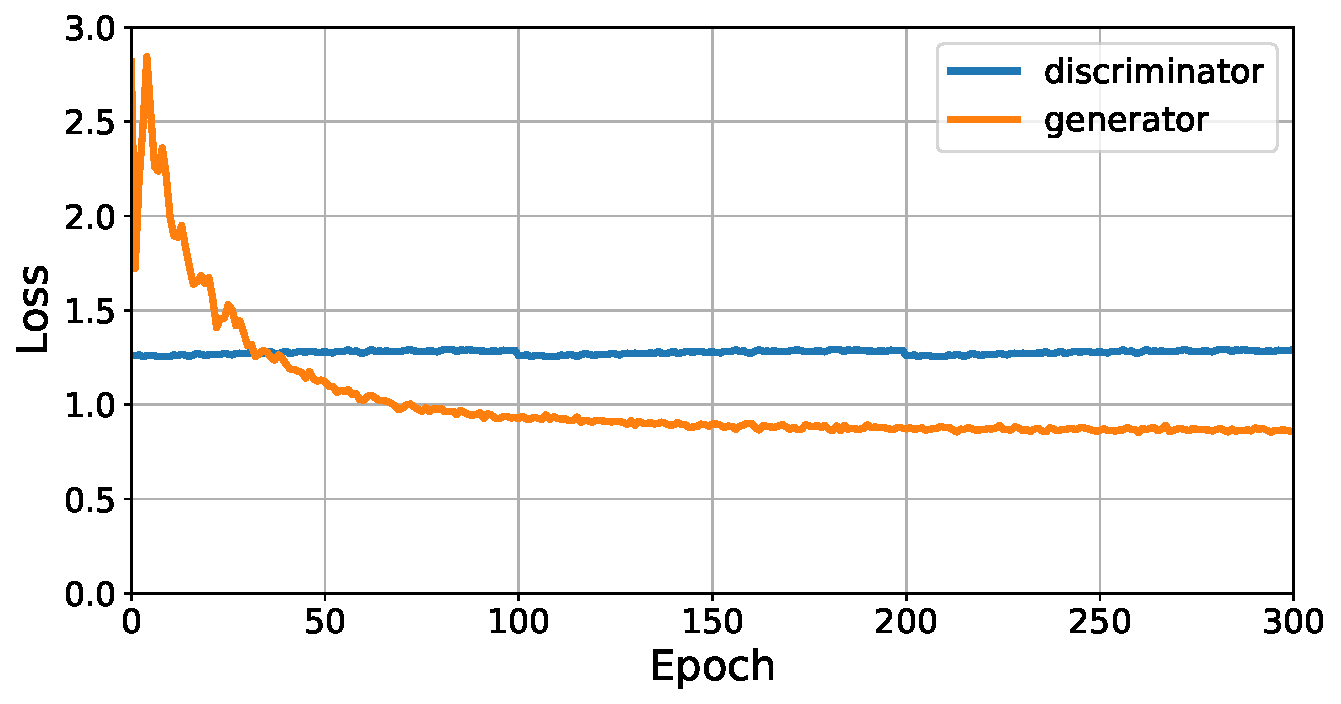
\includegraphics[width=0.75\textwidth]{figs/results/pytorch_vanilla_mnist_loss_0-299.pdf}
        \label{fig:results_pytorch_vanilla_mnist_loss}
    }
    \\
    \vspace{0.5cm}
    \subfigure[Incertezas]
    {
        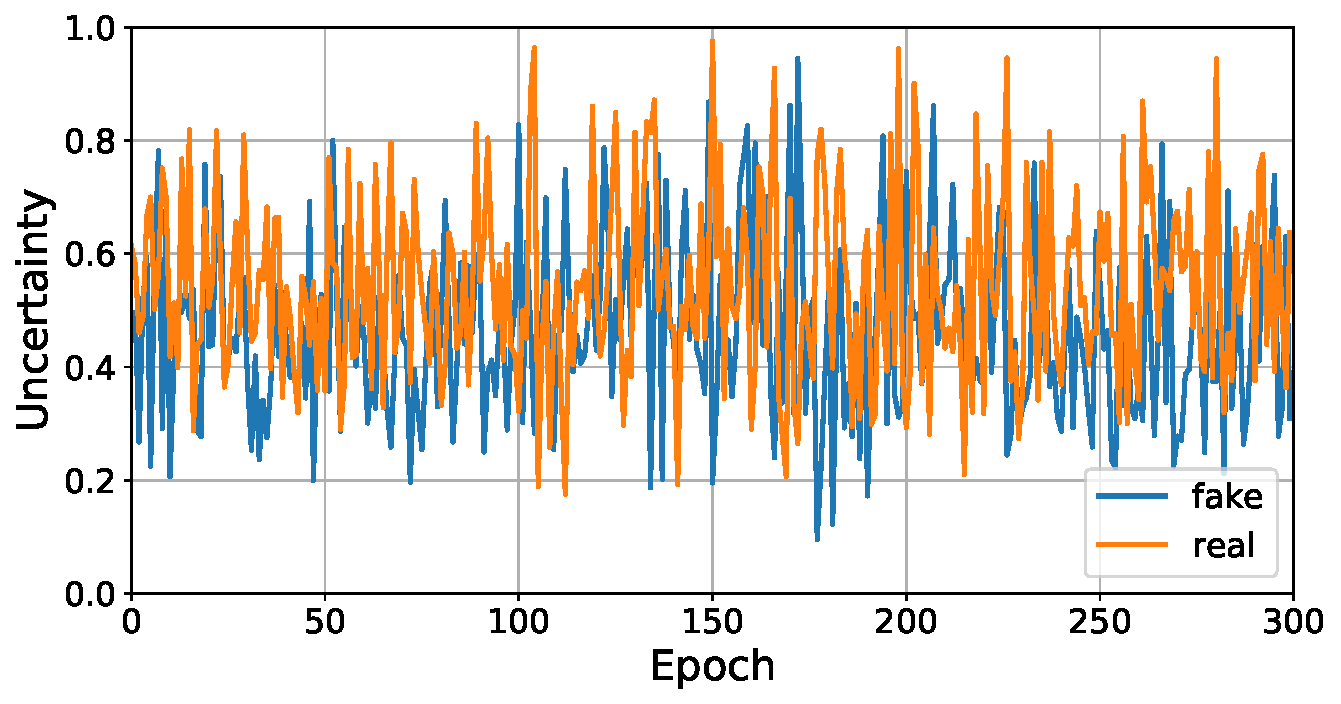
\includegraphics[width=0.75\textwidth]{figs/results/pytorch_vanilla_mnist_uncertainty_0-299.pdf}
        \label{fig:results_pytorch_vanilla_mnist_uncertainty}
    }
    \caption{Erros e incertezas da GAN \textit{Vanilla} para o \textit{dataset} MNIST em diferentes épocas.}
    \label{fig:results_pytorch_vanilla_mnist_scores}
\end{figure}